\section{Reinforcement learning}

%% The environment {{{
\subsection{The environment}

For the environment, the cliff walking with a size of $12\times4$ was chosen.
Specifically, a modified version of caburu's \verb|gym-cliffwalking|\cite{cliffwalking} is used.
Two main modifications have been made to the original code:
\begin{itemize}
	\item Originally, the state-space had a size of 48, though 10 of these are not real states.
		The cliff states were excluded.
	\item Rendering has been added.
\end{itemize}
So the environment has a state-space of size 38,
and an action-space of size 4 (right, down, left, up).

%% }}}

%% {{{ Model based methods
\subsection{Model based methods}

\subsubsection{Model generating}

Firstly, the model has been generated, which is basically a database of transitions and
rewards. $\fn{m}: \mathbb{X}\times\mathbb{A}\rightarrow\mathbb{R}\times\mathbb{X}$,
where $\mathbb{X}$ is the state-space and $\mathbb{A}$ is the action-space. A random
policy was used here. A figure of this can be seen running
\verb|3-Reinforcement_learning/show_scene.py| (taking the given action in the given state,
on the left, the numbers mean the rewards, on the right, the next states).

\subsubsection{Linear programming}

The optimal solution is given by linear programming.
Let $\fn{V}$ be an arbitrary value-function.
The optimal $\fn{V}^*$ is obtained by minimizing $\sum\fn{V}_S$, given
\begin{equation}
	\fn{V}_S\geq\fn{g}
(S, A) + \beta\fn{V}_{S+1} \text{ and } \fn{V}_\text{goal}=0,
\end{equation}
where $\beta$ is the discount factor, and $\fn{g}(S, A)$ is the immediate reward.
The optimization is done with the python library \verb|cvxpy|.

The resulting optimal value-function can be seen on figure \ref{fig:LP}.

\subsubsection{Value iteration}

An iterative solution is using value iteration.
Start with and arbitrary value-function (all zeros in this case),
and repeatedly sweep through the state-space. For all the states
\begin{equation}\label{eq:VI}
	\fn{V}_S^{n+1} = \max\limits_{A\in\mathbb{A}}\brc{R + \beta\fn{V}_{S+1}^n},
\end{equation}
where $(S,A)\Rightarrow R$ and $(S,A)\Rightarrow S+1$
can be queried from the model.
Then, $\lim\limits_{n\rightarrow\infty}\fn{V}^n\rightarrow\fn{V}^*$.

The value-functions at some iterations are shown on figure \ref{fig:VI}.

\subsubsection{Policy iteration}\label{sssec:PI}

An other iterative method is policy iteration.
Here we start with an arbitrary policy, then we evaluate it by calculating its value-function.
This is done similarly to \ref{eq:VI}, only $A$ is not the one with the maximal reward,
but the one given by the current policy.

After this, we make the policy greedy with respect to the calculated value-function:
$\fn{p}(S)=\operatorname{argmax}\limits_{A\in\mathbb{A}}\brc{R + \beta\fn{V}_{S+1}}$.

The value-functions at some iterations are shown on figure \ref{fig:PI}.

The (euclidean) distances of both $\fn{V}_\text{VI}$ and $\fn{V}_\text{PI}$ from $\fn{V}^*$ are
shown on figure \ref{fig:dist-1}.

%% Figures {{{
\begin{multicols}{3}
\newlength{\figsize}
\setlength{\figsize}{.25\textwidth}
\begin{figure}[H]
	\centering
	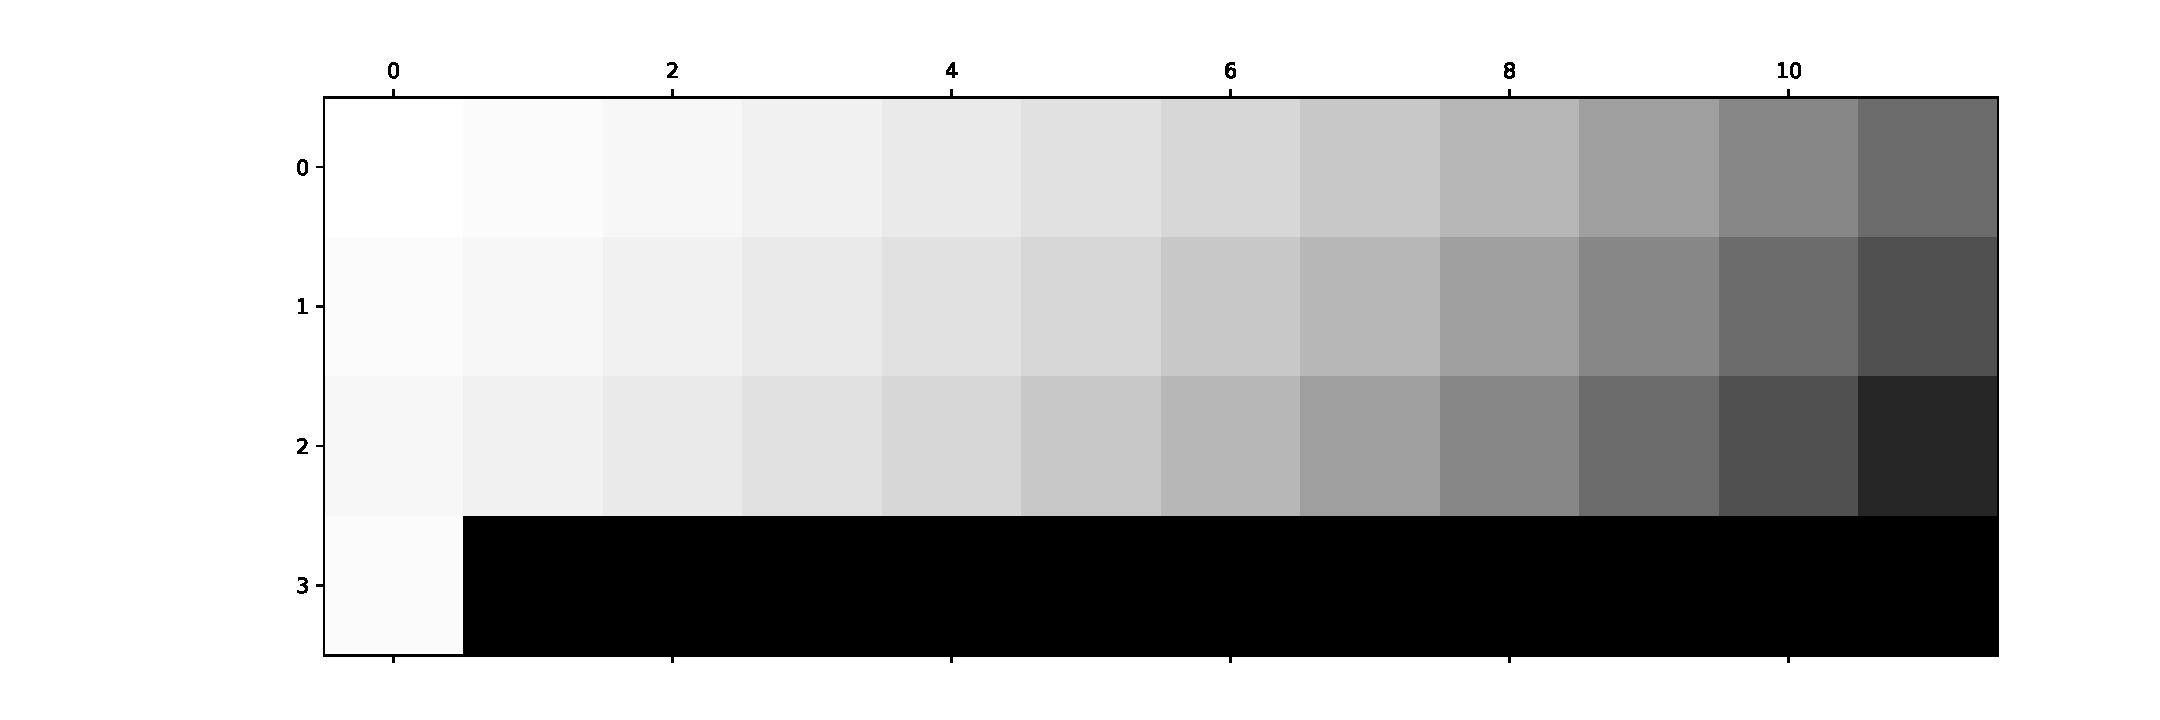
\includegraphics[width=\figsize, trim={54mm, 1cm, 2cm 15mm}, clip]{ex_III_1_plots_LP}
	\caption{Linear programming}
	\label{fig:LP}
\end{figure}
\columnbreak
\begin{figure}[H]
	\centering
	\begin{subfigure}{\figsize}
		\centering
		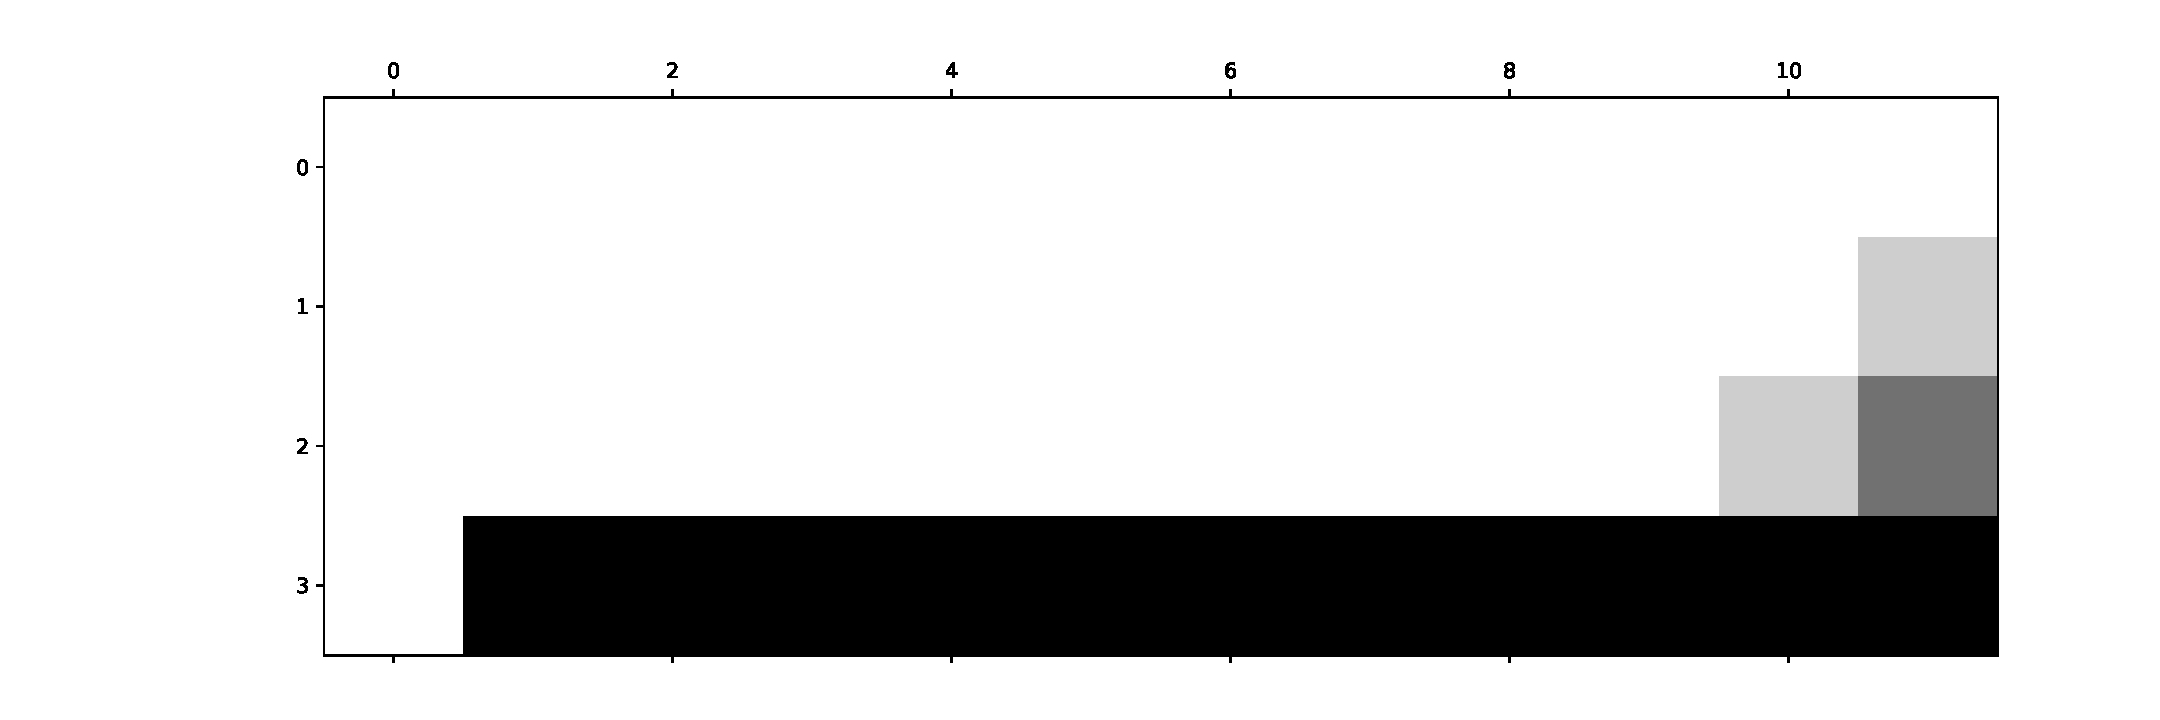
\includegraphics[width=\textwidth, trim={54mm, 1cm, 2cm 15mm}, clip]{ex_III_1_plots_VI_2}
		\caption{Iteration 2}
		\label{fig:ex_III_1_plots_VI_2}
	\end{subfigure}\\
	\begin{subfigure}{\figsize}
		\centering
		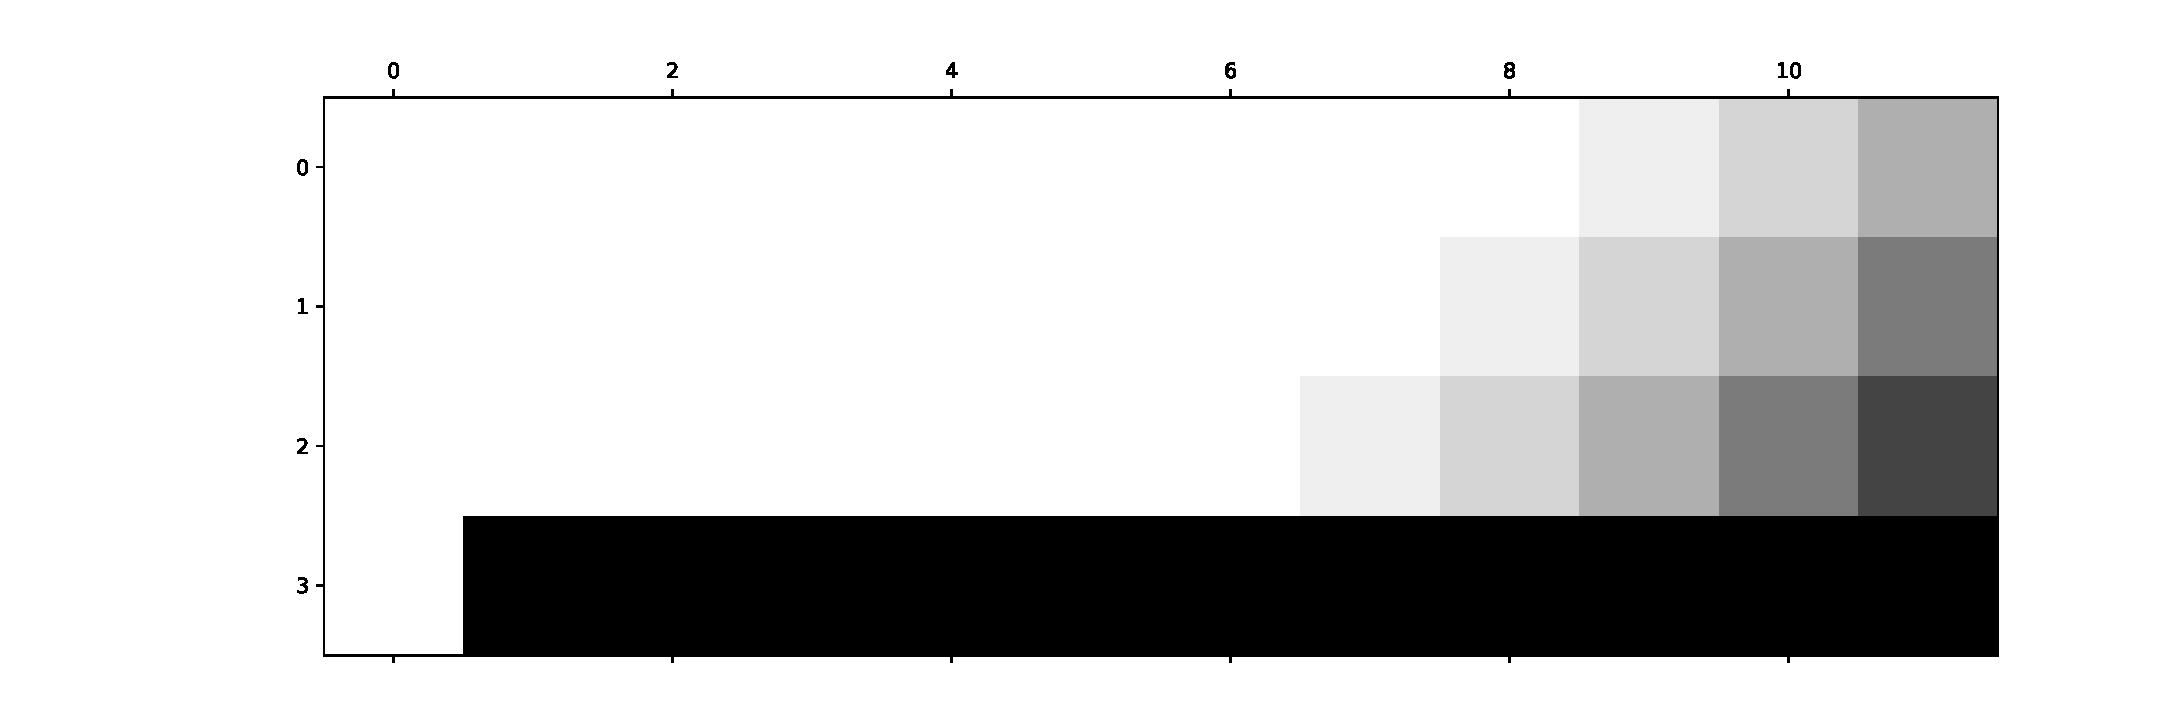
\includegraphics[width=\textwidth, trim={54mm, 1cm, 2cm 15mm}, clip]{ex_III_1_plots_VI_5}
		\caption{Iteration 5}
		\label{fig:ex_III_1_plots_VI_5}
	\end{subfigure}\\
	\begin{subfigure}{\figsize}
		\centering
		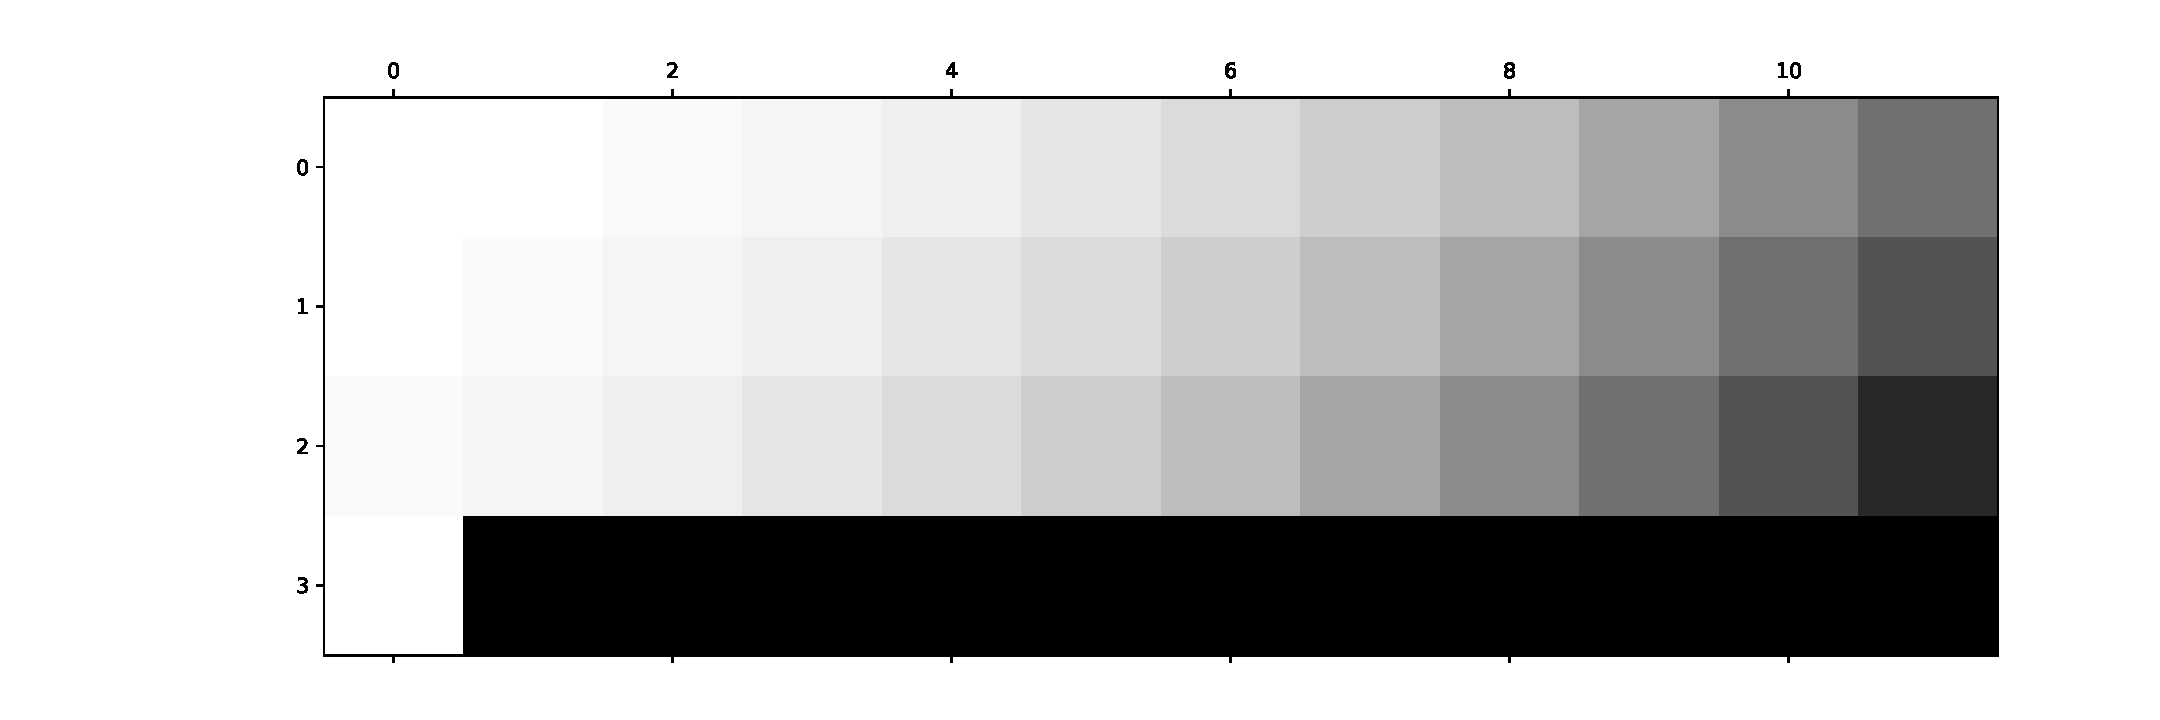
\includegraphics[width=\textwidth, trim={54mm, 1cm, 2cm 15mm}, clip]{ex_III_1_plots_VI_12}
		\caption{Iteration 12}
		\label{fig:ex_III_1_plots_VI_12}
	\end{subfigure}
	\caption{Value iteration}
	\label{fig:VI}
\end{figure}
\begin{figure}[H]
	\centering
	\begin{subfigure}{\figsize}
		\centering
		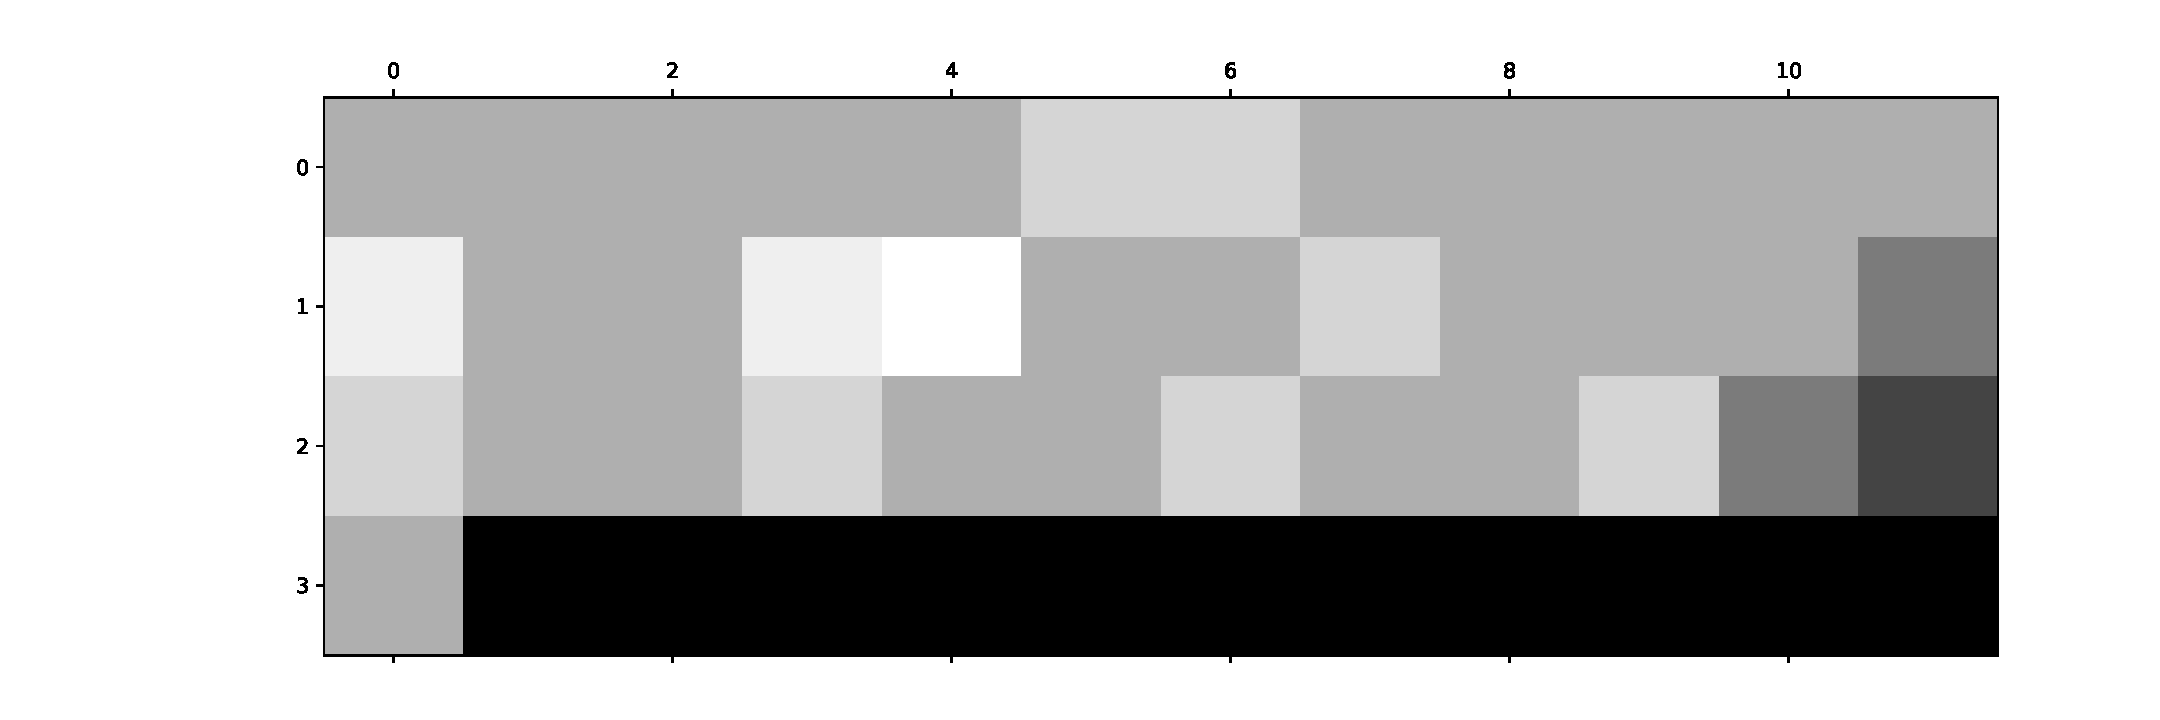
\includegraphics[width=\textwidth, trim={54mm, 1cm, 2cm 15mm}, clip]{ex_III_1_plots_PI_2}
		\caption{Iteration 2}
		\label{fig:ex_III_1_plots_PI_2}
	\end{subfigure}\\
	\begin{subfigure}{\figsize}
		\centering
		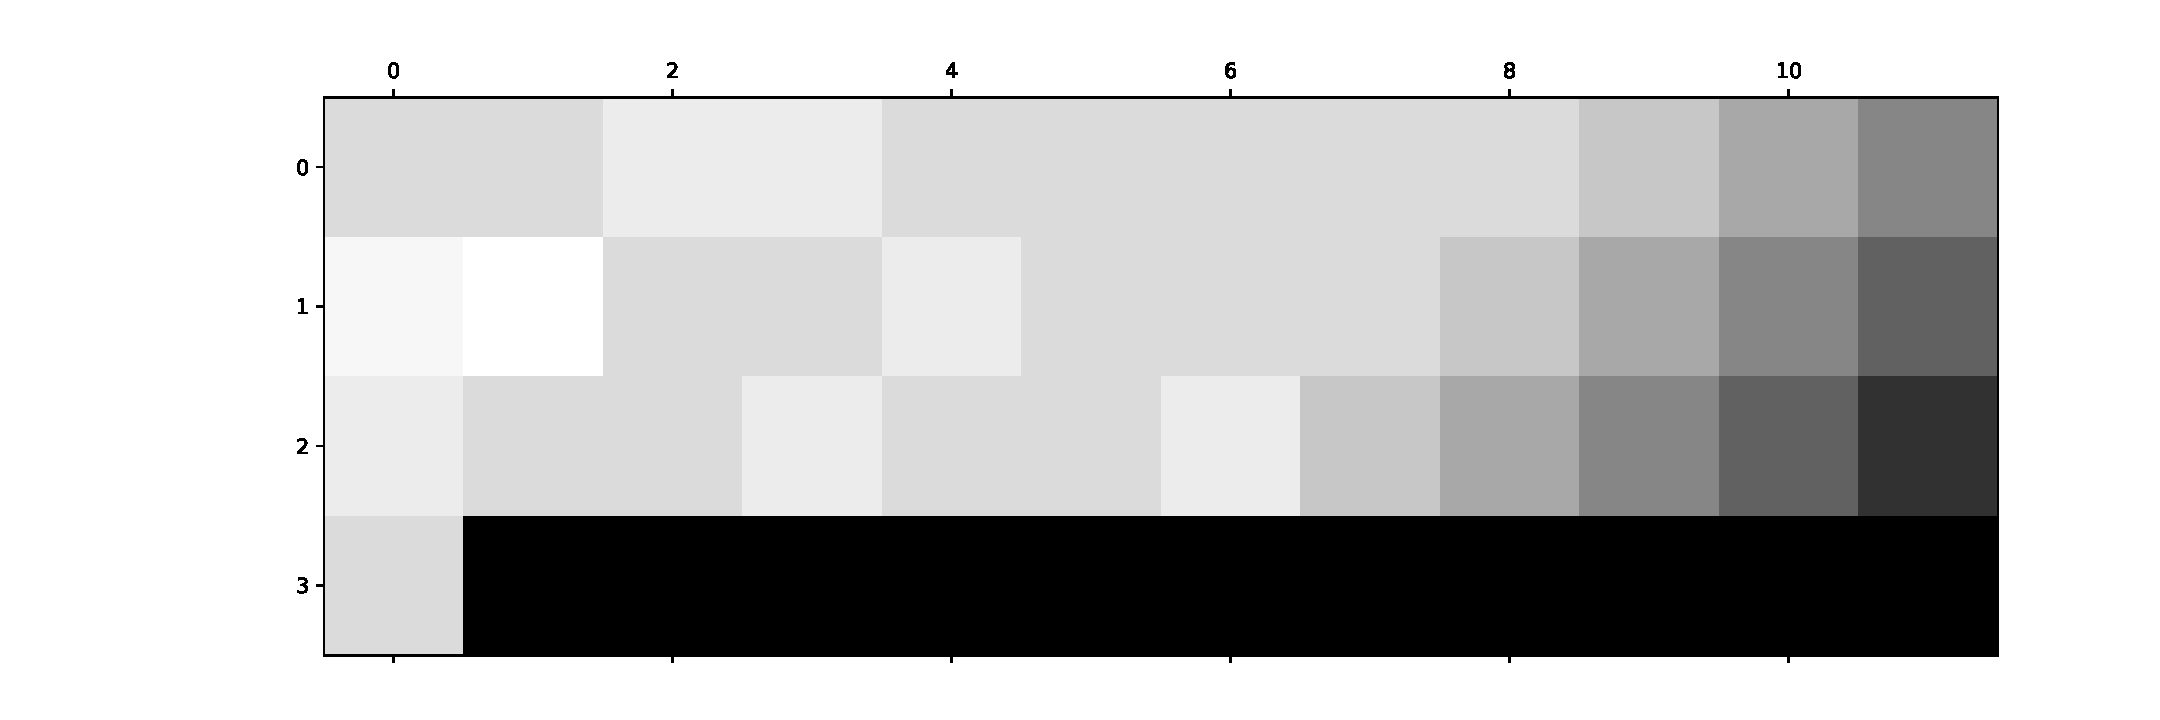
\includegraphics[width=\textwidth, trim={54mm, 1cm, 2cm 15mm}, clip]{ex_III_1_plots_PI_5}
		\caption{Iteration 5}
		\label{fig:ex_III_1_plots_PI_5}
	\end{subfigure}\\
	\begin{subfigure}{\figsize}
		\centering
		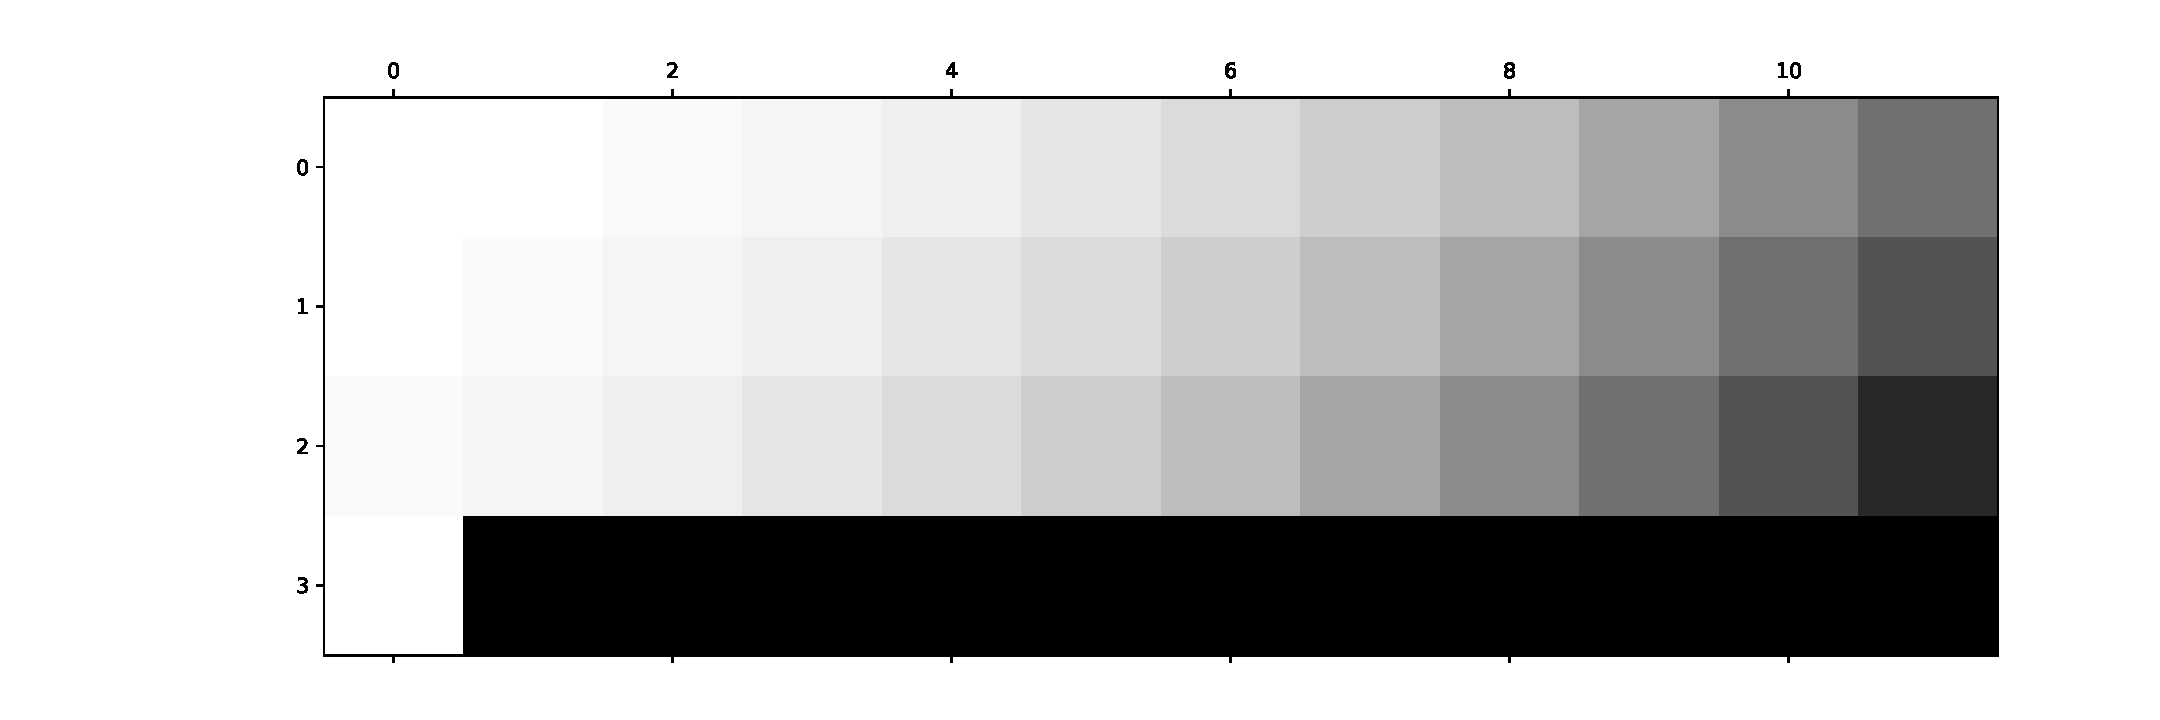
\includegraphics[width=\textwidth, trim={54mm, 1cm, 2cm 15mm}, clip]{ex_III_1_plots_PI_12}
		\caption{Iteration 12}
		\label{fig:ex_III_1_plots_PI_12}
	\end{subfigure}
	\caption{Policy iteration}
	\label{fig:PI}
\end{figure}
\end{multicols}
%% }}}

%% }}}

%% Model-free methods {{{
\subsection{Model-free methods}

In this section, online Q-learning is going to be implemented.
The update rule of Watkins' Q-learning is as follows:
\begin{equation}
	\fn{Q}_{n+1}(S,A)=(1-\gamma_n)\,Q_n(S, A) + \gamma_n\,(R + \beta\,\max\limits_{B\in\mathbb{A}}\fn{Q}_n(\widetilde{S},B)),
\end{equation}
where $\gamma_n=\frac{1}{n+1}$ is the learning rate at step $n$, and $\widetilde{S}$ is the next state.
At every step, $A=\fn{p}(S)$ is given by the policy.

Three policies are going to be put to test.

Firstly, the random policy, which just generates random actions for every state.

Second, the $\epsilon$-greedy policy. This acts greedily (see paragraph \ref{sssec:PI}),
most of the time, with acts randomly with an $\epsilon$ probalility so as to
encourage exploration.

Lastly, the semi-greedy policy (called soft-max in the code) basically acts randomly
if it doesn't have a much better choice. The exact probability of choosing action $A$
is given by
\begin{equation}
	\mathbb{P}\brc{\pi_n(S)=A} =
	\frac{\exp\brc{\fn{Q}_n(S, A)/\tau}}
	{\sum\limits_{B\in\mathbb{A}}\exp\brc{\fn{Q}_n(S, B)/\tau}},
\end{equation}
where $\tau$ is the so-called Boltzmann-temperature, which influences
the randomness of the policy.

For all three policies, the value-functions at some iterations are shown
on figures \ref{fig:random}, \ref{fig:e-greedy} and \ref{fig:semi-greedy}.

Also the distances of these policies' value-functions from the optimal one
can be seen in figure \ref{fig:dist-2}
The sums of the rewards received are also shown in figure \ref{fig:rewards}.

%% Figures {{{
\begin{multicols}{3}
	\setlength{\figsize}{.25\textwidth}
	\begin{figure}[H]
		\centering
		\begin{subfigure}{\figsize}
			\centering
			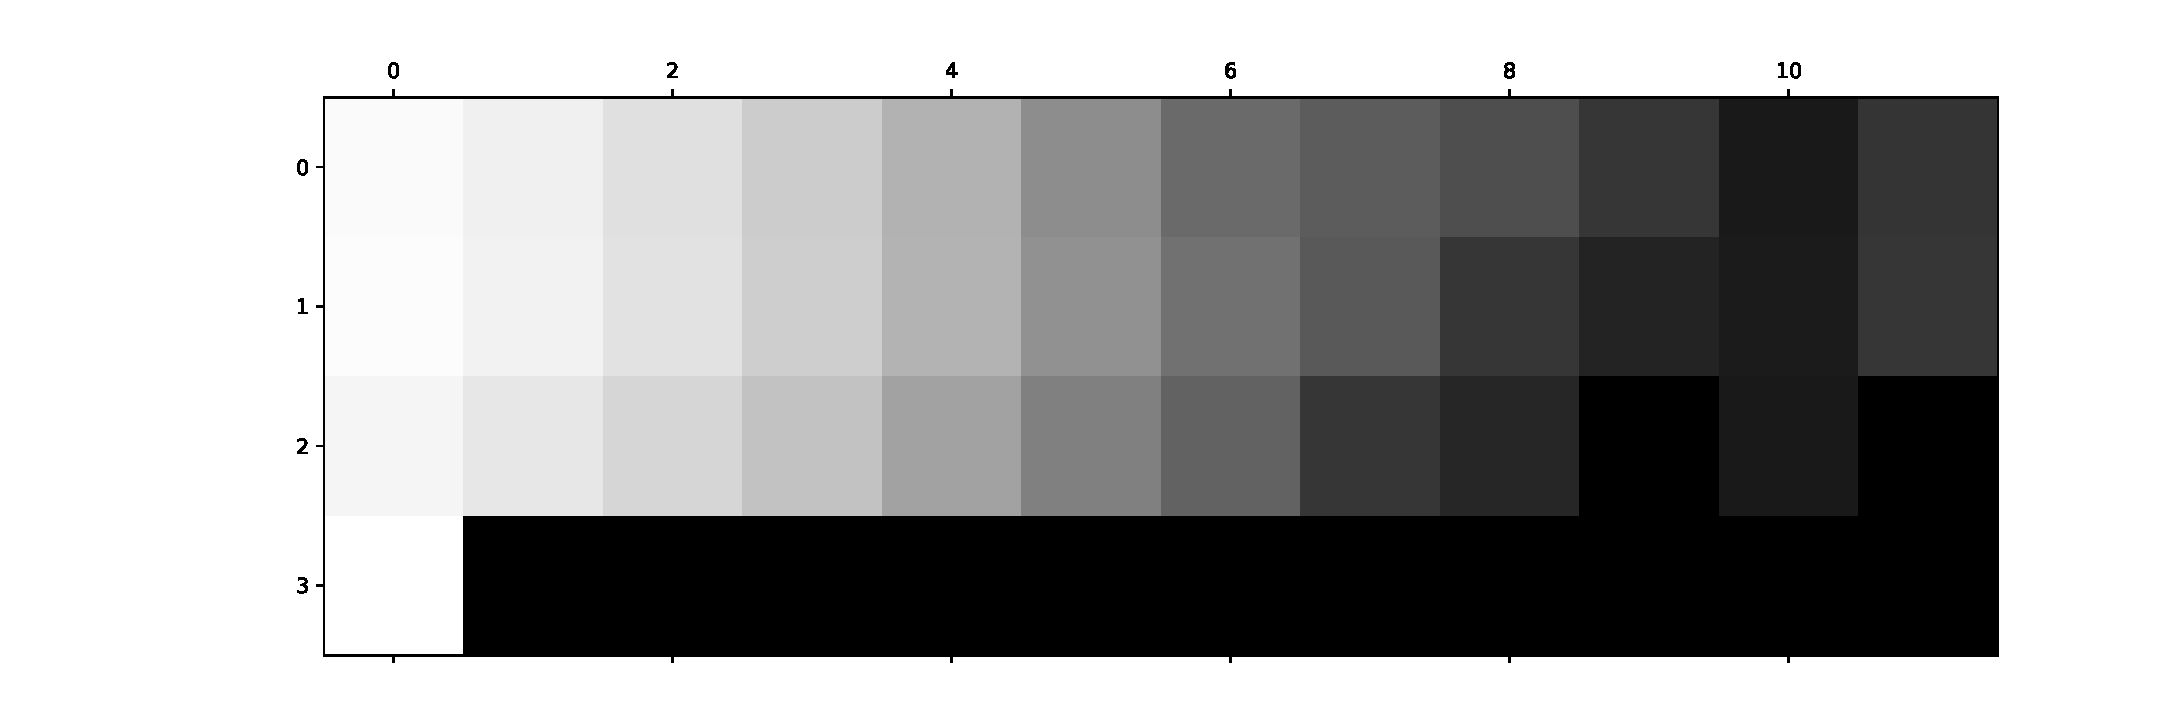
\includegraphics[width=\textwidth, trim={54mm, 1cm, 2cm 15mm}, clip]{ex_III_2_plots_random_2}
			\caption{Iteration 2}
			\label{fig:ex_III_2_plots_random_2}
		\end{subfigure}\\
		\begin{subfigure}{\figsize}
			\centering
			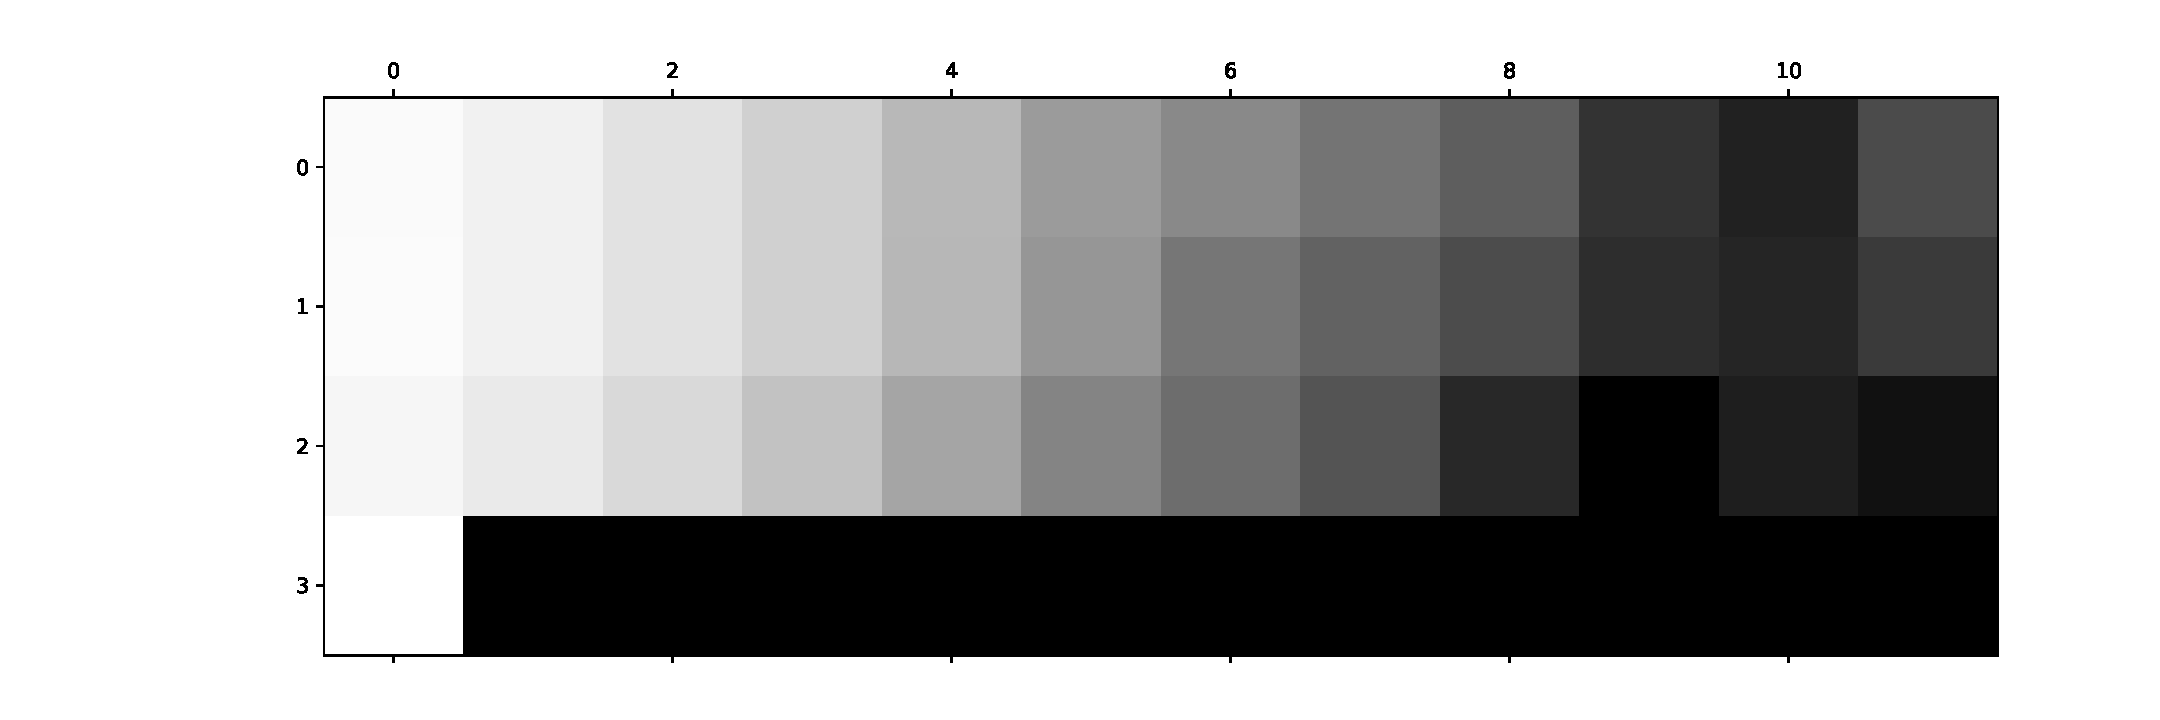
\includegraphics[width=\textwidth, trim={54mm, 1cm, 2cm 15mm}, clip]{ex_III_2_plots_random_5}
			\caption{Iteration 5}
			\label{fig:ex_III_2_plots_random_5}
		\end{subfigure}\\
		\begin{subfigure}{\figsize}
			\centering
			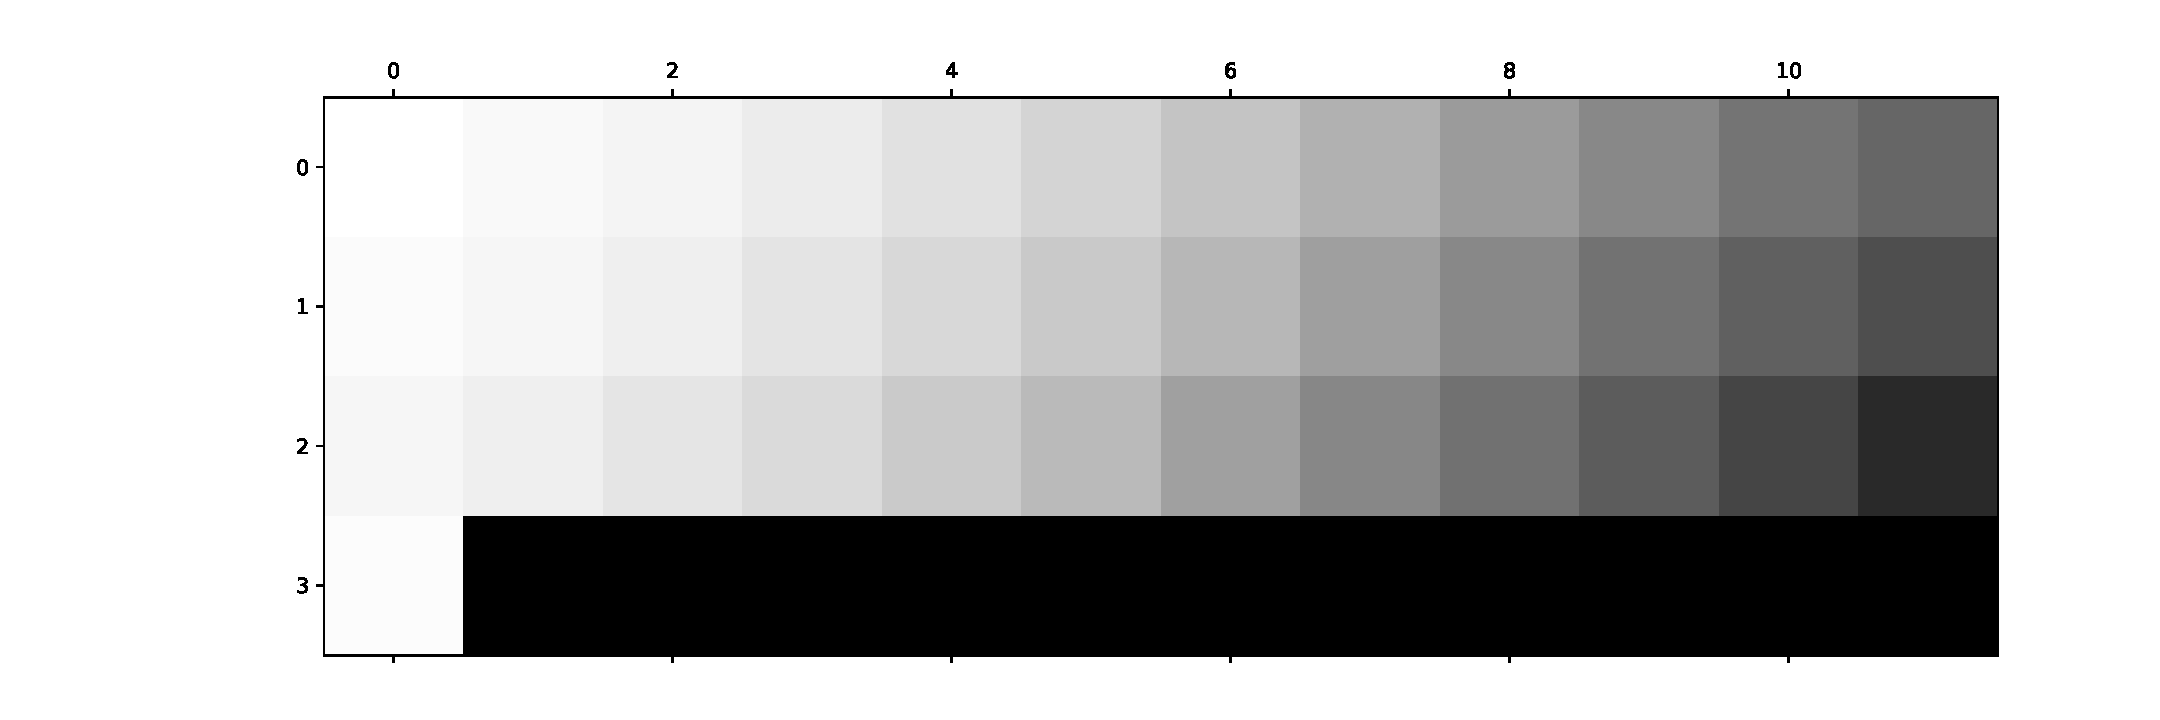
\includegraphics[width=\textwidth, trim={54mm, 1cm, 2cm 15mm}, clip]{ex_III_2_plots_random_30}
			\caption{Iteration 30}
			\label{fig:ex_III_2_plots_random_30}
		\end{subfigure}
		\caption{Random policy}
		\label{fig:random}
	\end{figure}
	\columnbreak

	\begin{figure}[H]
		\centering
		\begin{subfigure}{\figsize}
			\centering
			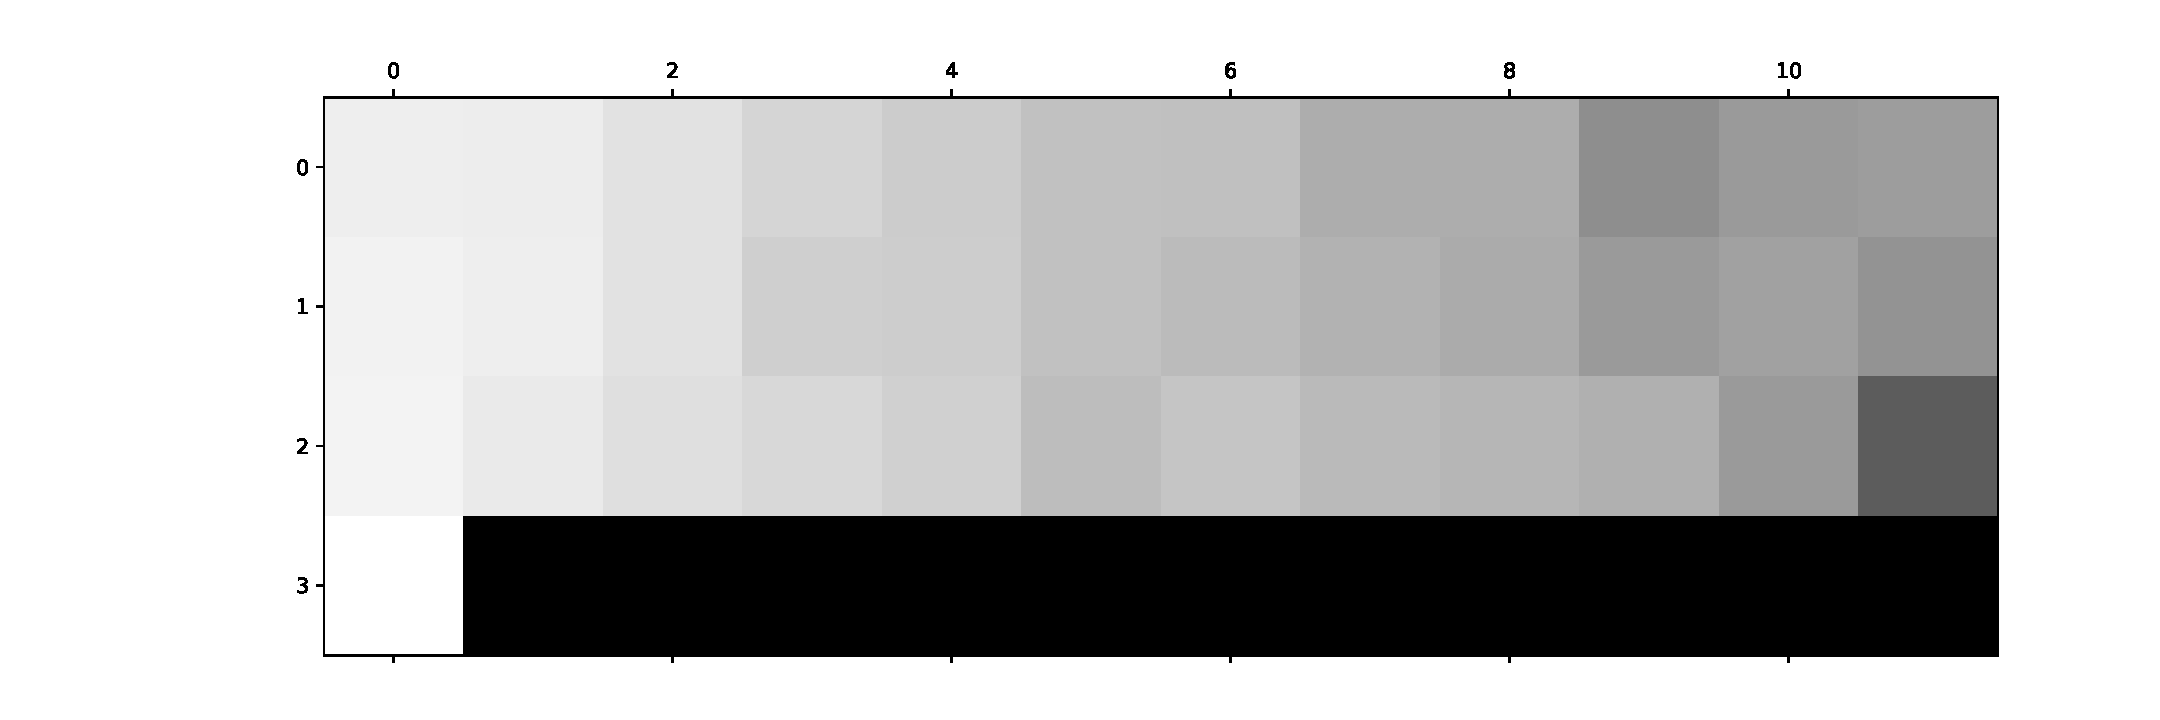
\includegraphics[width=\textwidth, trim={54mm, 1cm, 2cm 15mm}, clip]{ex_III_2_plots_e-greedy_2}
			\caption{Iteration 2}
			\label{fig:ex_III_2_plots_e-greedy_2}
		\end{subfigure}\\
		\begin{subfigure}{\figsize}
			\centering
			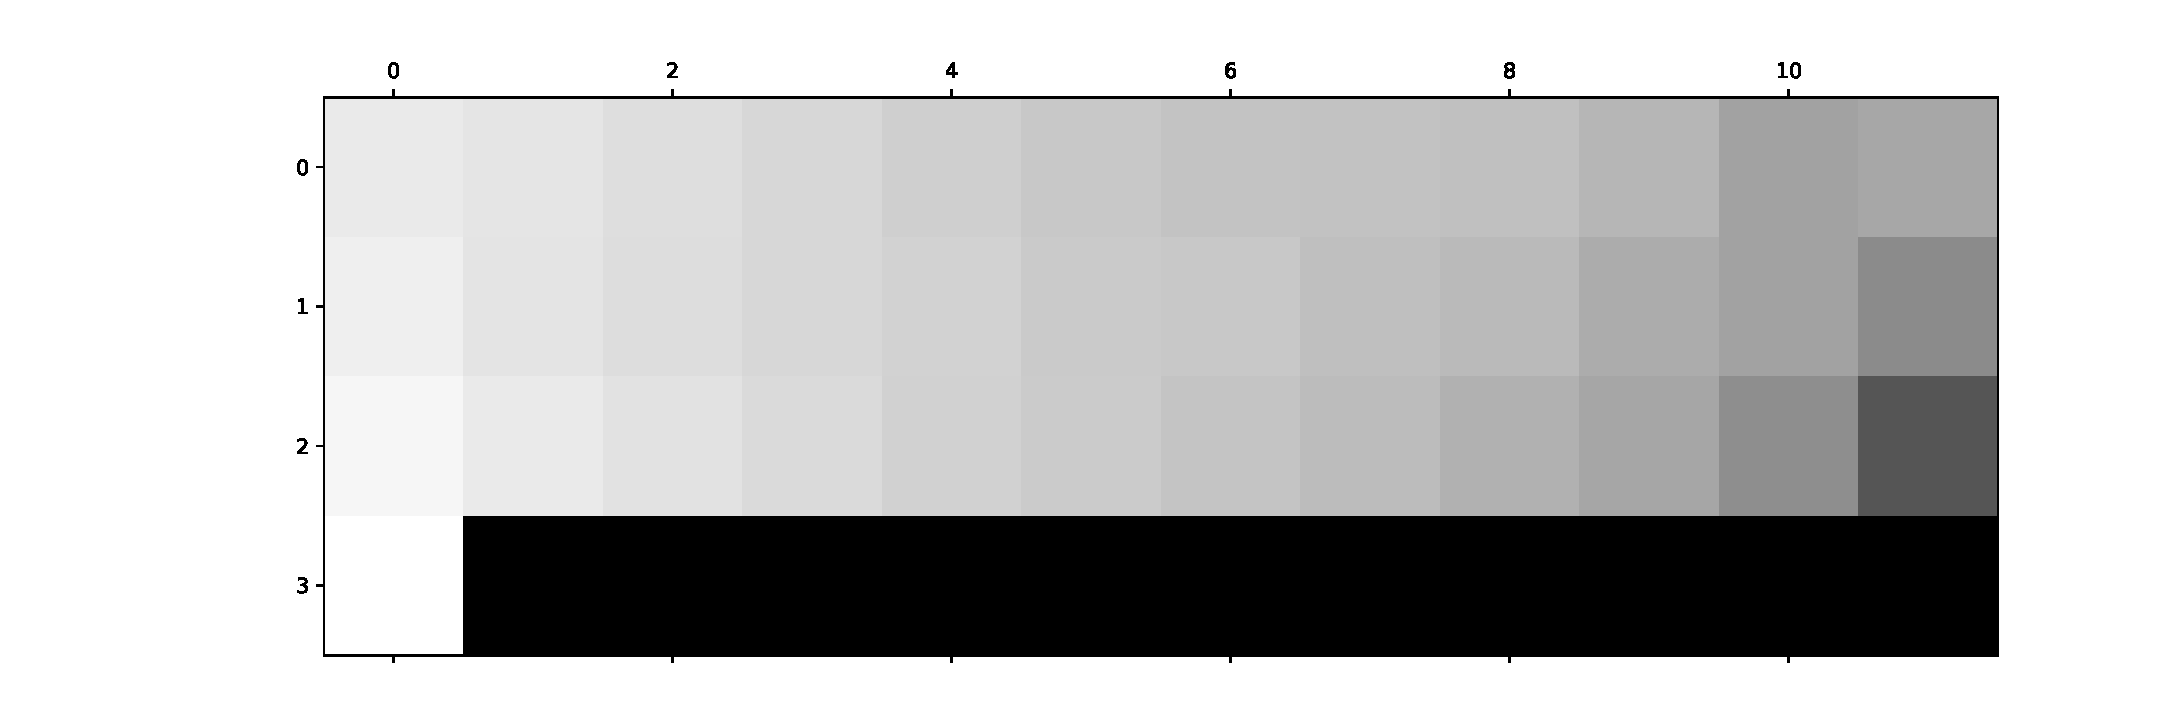
\includegraphics[width=\textwidth, trim={54mm, 1cm, 2cm 15mm}, clip]{ex_III_2_plots_e-greedy_5}
			\caption{Iteration 5}
			\label{fig:ex_III_2_plots_e-greedy_5}
		\end{subfigure}\\
		\begin{subfigure}{\figsize}
			\centering
			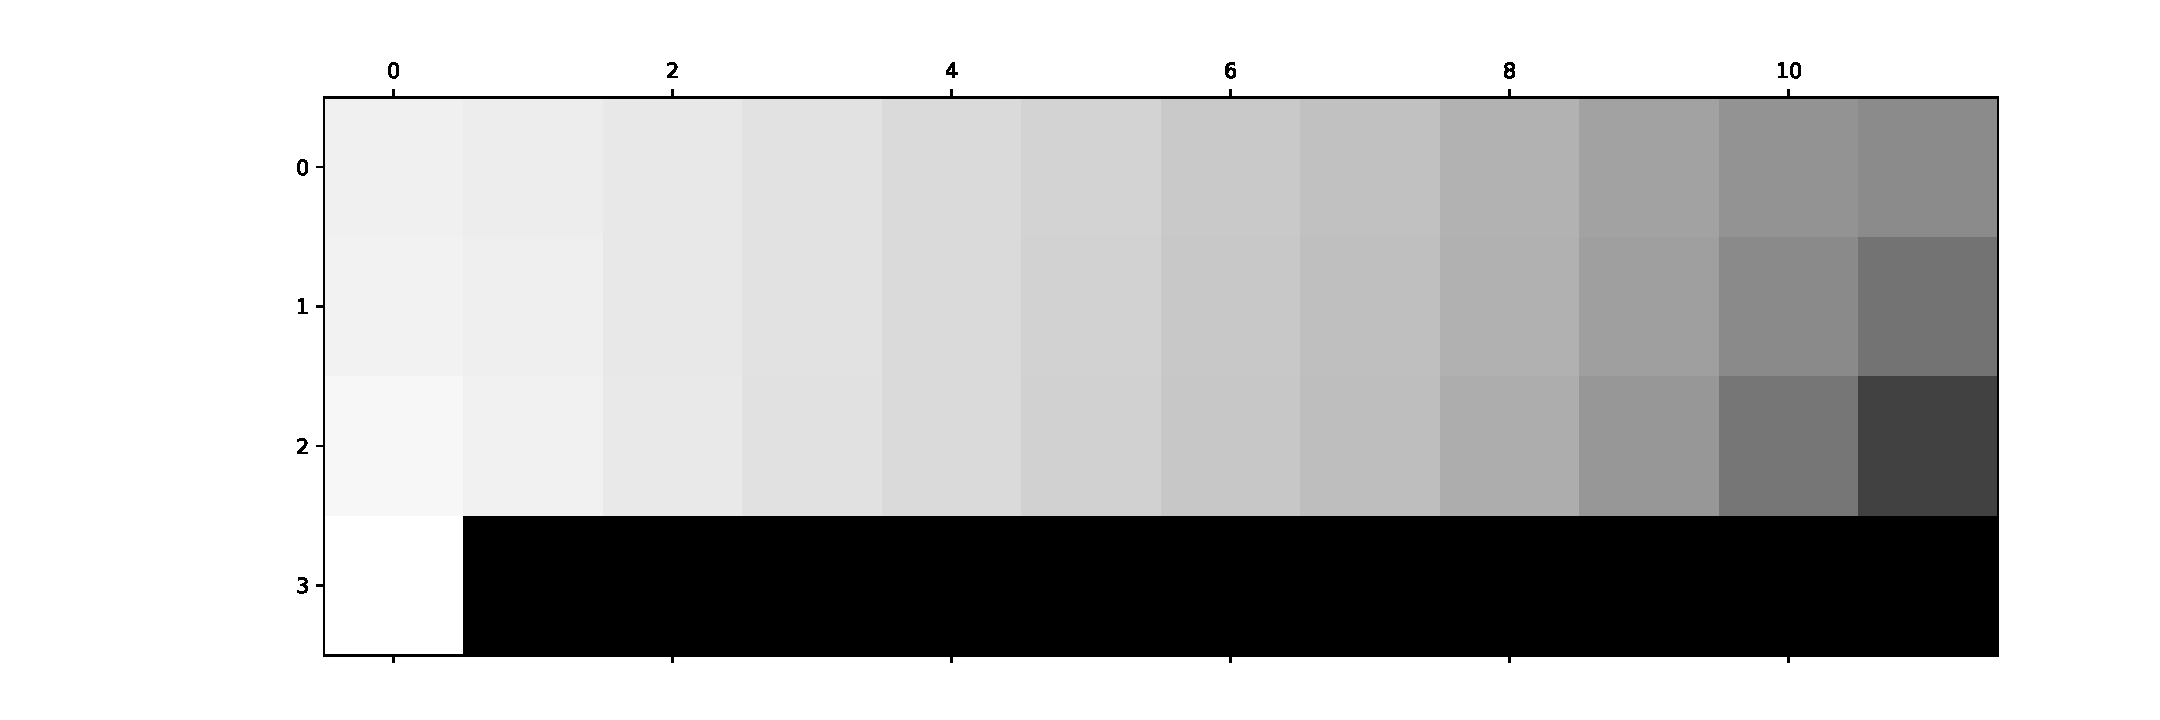
\includegraphics[width=\textwidth, trim={54mm, 1cm, 2cm 15mm}, clip]{ex_III_2_plots_e-greedy_30}
			\caption{Iteration 30}
			\label{fig:ex_III_2_plots_e-greedy_30}
		\end{subfigure}
		\caption{$\epsilon$-greedy policy}
		\label{fig:e-greedy}
	\end{figure}
	\columnbreak

	\begin{figure}[H]
		\centering
		\begin{subfigure}{\figsize}
			\centering
			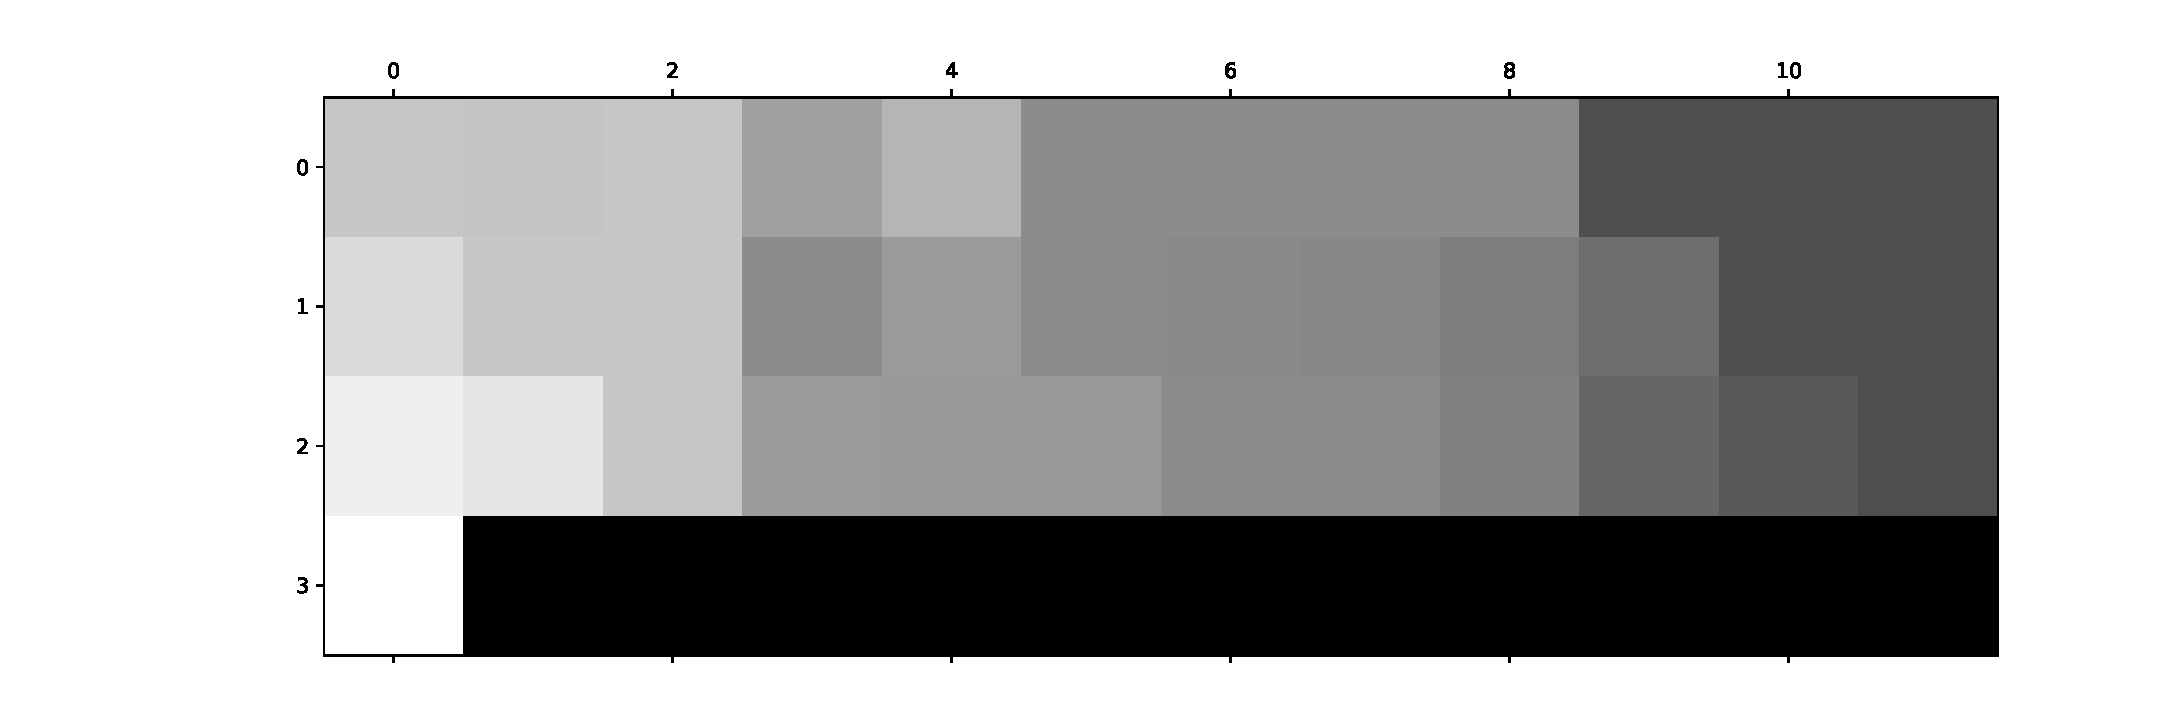
\includegraphics[width=\textwidth, trim={54mm, 1cm, 2cm 15mm}, clip]{ex_III_2_plots_soft-max_2}
			\caption{Iteration 2}
			\label{fig:ex_III_2_plots_soft-max_2}
		\end{subfigure}\\
		\begin{subfigure}{\figsize}
			\centering
			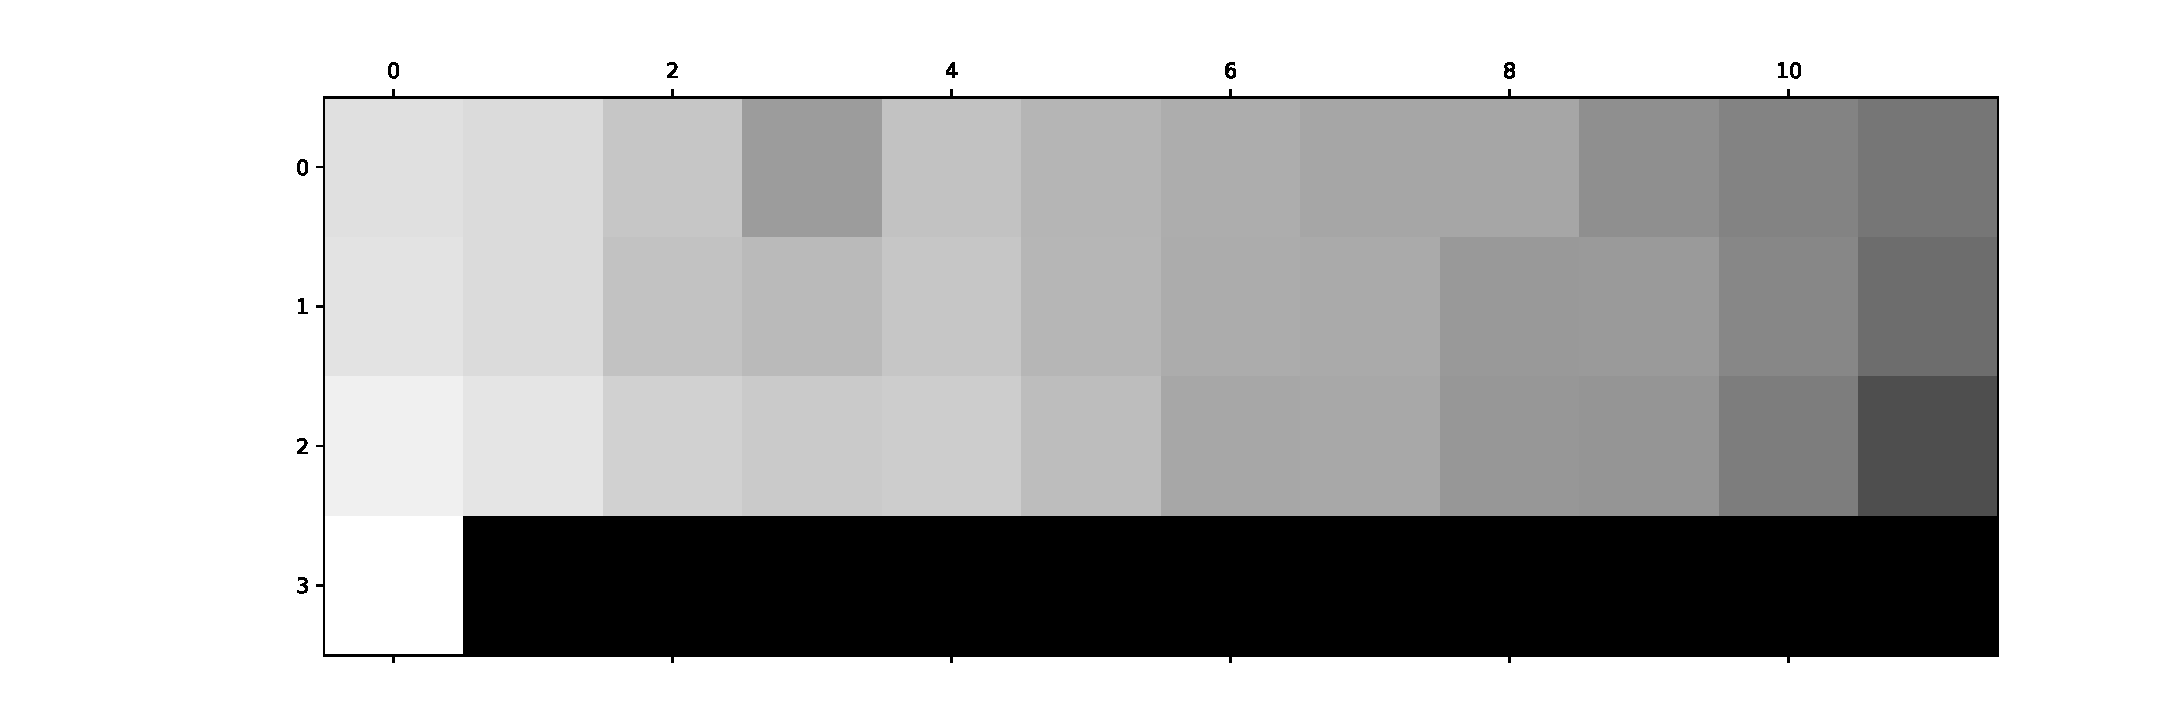
\includegraphics[width=\textwidth, trim={54mm, 1cm, 2cm 15mm}, clip]{ex_III_2_plots_soft-max_5}
			\caption{Iteration 5}
			\label{fig:ex_III_2_plots_soft-max_5}
		\end{subfigure}\\
		\begin{subfigure}{\figsize}
			\centering
			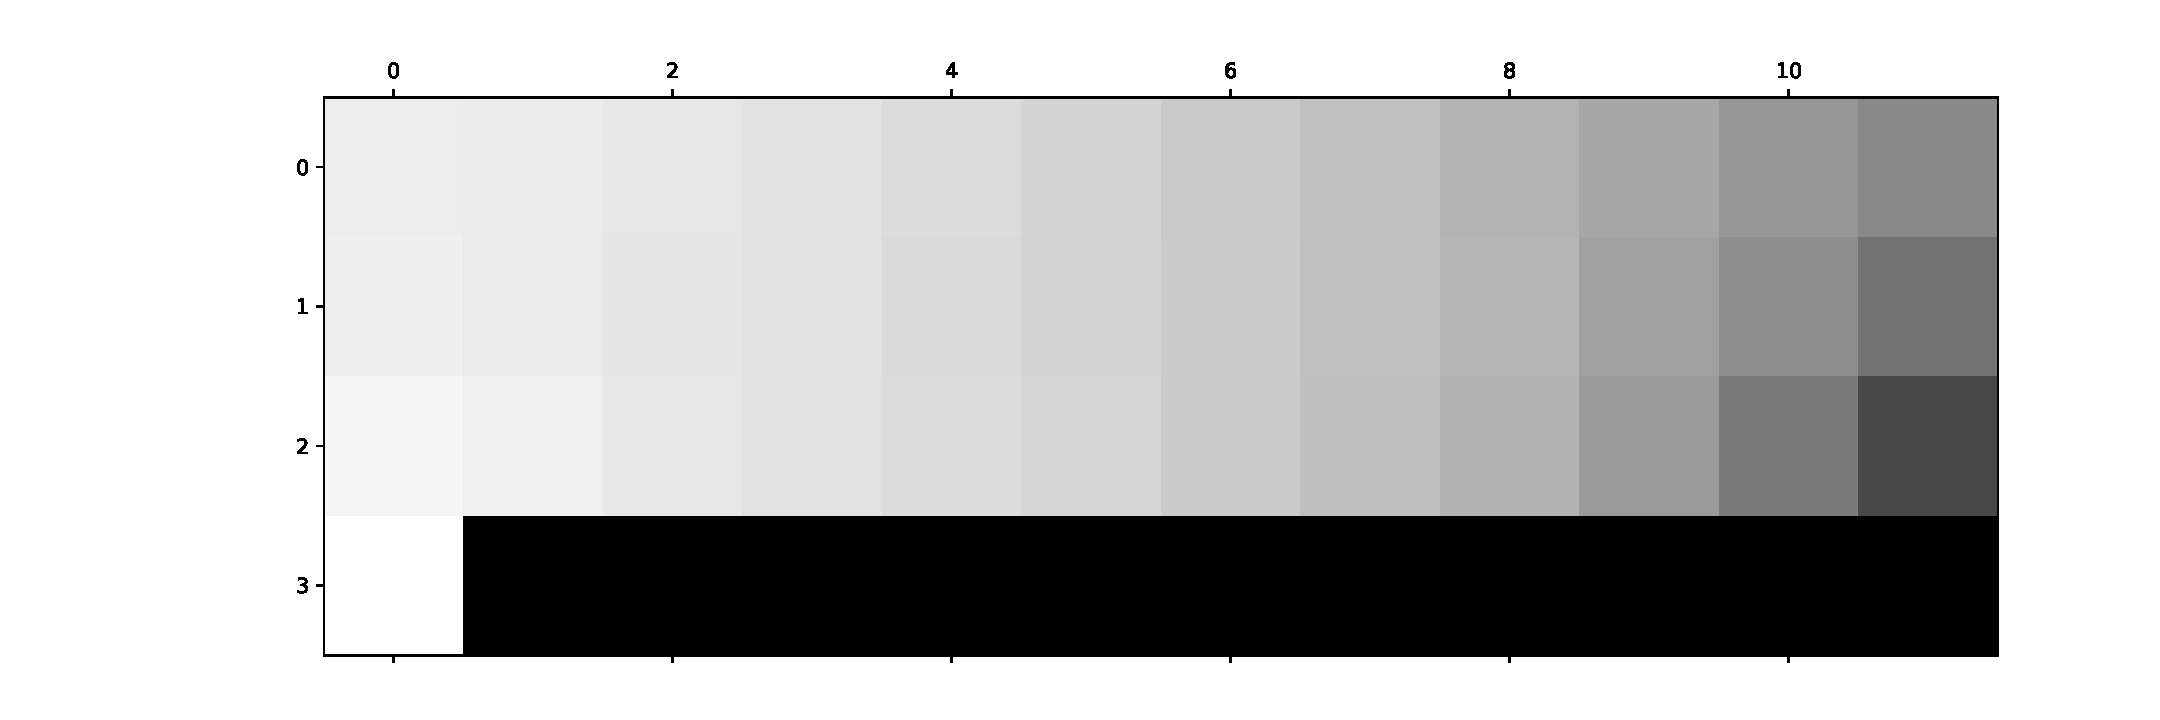
\includegraphics[width=\textwidth, trim={54mm, 1cm, 2cm 15mm}, clip]{ex_III_2_plots_soft-max_30}
			\caption{Iteration 30}
			\label{fig:ex_III_2_plots_soft-max_30}
		\end{subfigure}
		\caption{Semi-greedy policy}
		\label{fig:semi-greedy}
	\end{figure}
\end{multicols}

\begin{figure}[H]
	\centering
	\begin{subfigure}{.32\textwidth}
		\centering
		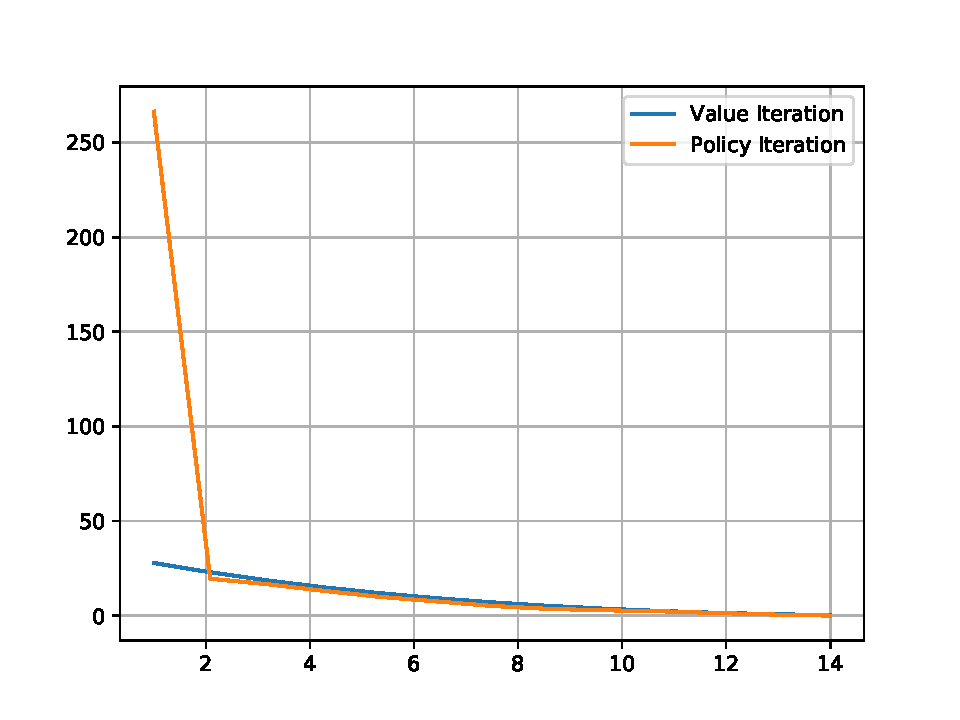
\includegraphics[width=\textwidth]{ex_III_1_plots_dist}
		\caption{Model-based}
		\label{fig:dist-1}
	\end{subfigure}
	\begin{subfigure}{.32\textwidth}
		\centering
		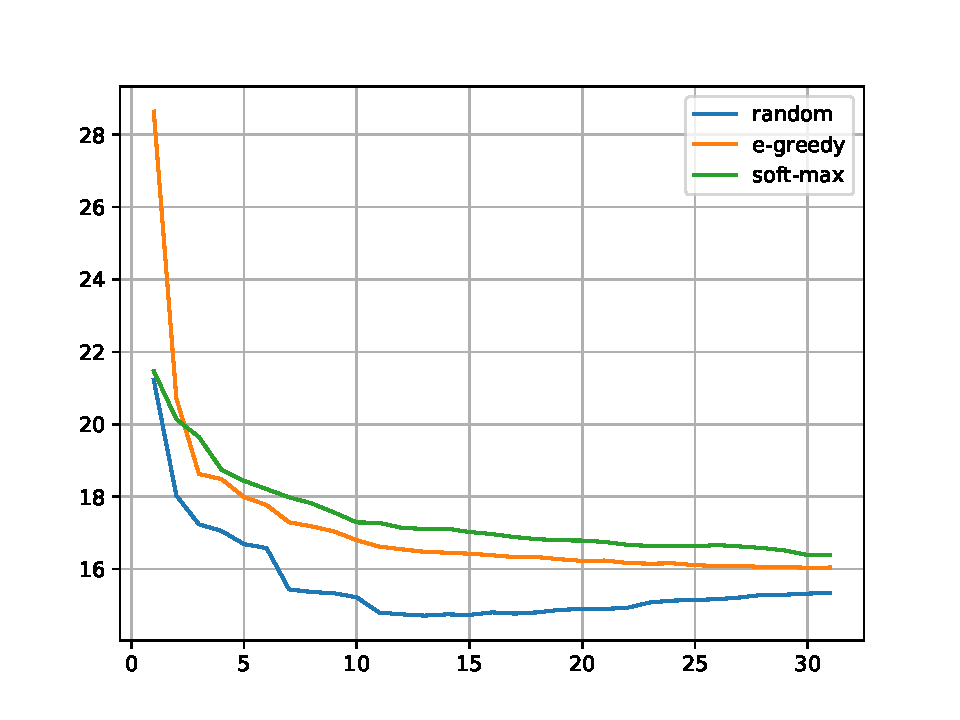
\includegraphics[width=\textwidth]{ex_III_2_plots_soft-max_dists}
		\caption{Model-free}
		\label{fig:dist-2}
	\end{subfigure}
	\begin{subfigure}{.32\textwidth}
		\centering
		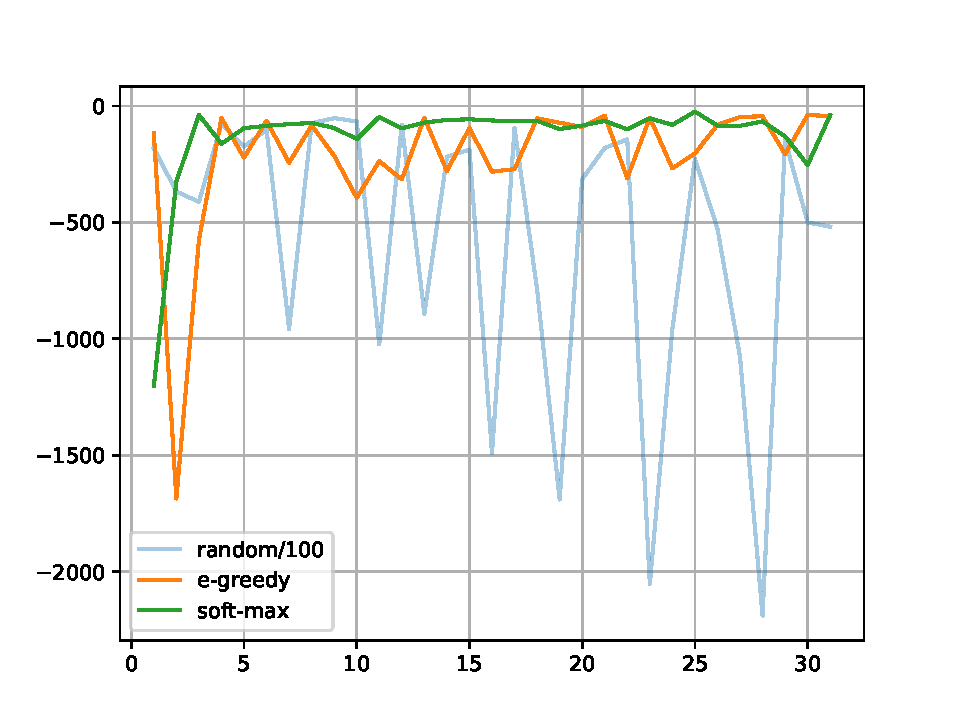
\includegraphics[width=\textwidth]{ex_III_2_plots_soft-max_rewards}
		\caption{Rewards (model-free)}
		\label{fig:rewards}
	\end{subfigure}
	\caption{Distance from the optimal value-function, and rewards of policies}
\end{figure}

%% }}}

%% }}}
